\subsection{Optimization of the intensity of the beams}
\subsubsection{Preliminary results}
We have already tried several methods : active set method, penalty method
and simulated annealing.We used these methods with a  two dimensional code for 
neutral particles instead of the three dimensional photon-electron problem. 

\paragraph{Active method}
The first method we tried was a variant of the active set method inspired by
\cite{dose-volume}. The algorithm works as follow :
\begin{itemize}
\item Step 1 : Optimize the dose without any constraint.
\item Step 2 : Sort the voxel in the healthy organs by their received dose
from a low dose to a high dose.
\item Step 3 : Apply the constraint $D_{ijk}<\delta_{ijk}$ on the $(1-\gamma)
N$ voxels with the lowest dose ($N$ is the number of voxels for the organ) for
each organ,
\item Step 4 : Solve the constrained optimization problem using the active set
method.
\item Step 5 : Go back to Step 3 until the solution cannot be improved
anymore. 
\end{itemize}
This method is rapid but does not give reliable results when the solution of the
constrained problem is very different from the solution of the unconstrained
problem. 

\paragraph{Penalty method}
Instead of minimizing a constrained optimization problem, we solve an unconstrained problem :
\begin{equation}
\min Q_{\mu} (x) = f(x) + \frac{1}{2\mu} \|g(x)\|^2 + \frac{1}{2\mu} \|\[h(x)\]^-\|^2
\end{equation}
where :
\begin{equation}
\[h(x)\]^- = \min \{0,h(x)\}
\end{equation}
We decrease the value of the parameter $\mu$ during the optimization process.
We have the following objective function :
\begin{equation}
f = \sum_{(i,j)\in \mathcal T} \(D_{ijk} - \delta_{ijk}\)^2
\end{equation}
The constraints are given by :
\begin{align}
&h_1 = \gamma - \sum_{ijk \in \mathcal{D}} \frac{V_{ijk}}{V} \nu \(D_{ijk} -
\delta_{ijk}\) \geq 0 \label{dv}\\
&h_2 = D_{ijk} \geq 0
\end{align}
Thus, we have the following quadratic relaxation :
\begin{equation}
Q_{\mu} = \sum_{(i,j,k)\in \mathcal T} \(D_{ijk} - \delta_{ijk}\)^2 +
\frac{1}{2\mu} \(\[\gamma - \sum_{(i,j,k) \in \mathcal{D}} \frac{V_{ijk}}{V}
\nu \(D_{ijk} - \delta_{ijk}\)\]^-\)^2 + \frac{1}{2\mu} \(\[D_{ijk}\]^-\)^2
\end{equation}
If we want to use the steepest descent or Newton's method to solve the
previous problem, we need to take the derivative of the Heaviside function and
this is an issue because the derivative is a Dirac distribution. Therefore, 
we use the following \hbox{approximation :}
\begin{equation}
\nu (x) = \frac{1}{1+e^{-2\alpha x}}
\end{equation}
where $k$ is a large constant.
The gradient of the quadratic relaxation is :
\begin{equation}
\begin{split}
\bn Q_{\mu} &= \sum_{(i,j,k) \in \mathcal{T}} 2 \(D_{ijk} - \delta_{ijk}\) \bn
D_{ijk} + \frac{1}{\mu} \(\[\gamma - \sum_{(i,j,k) \in
\mathcal{D}}\frac{V_{ijk}}{V} \frac{1}{1+e^{-2k\(D_{ijk} - \delta_{ijk}\)}}\]^-\) \times\\
&\(\sum_{(i,j,k)\in \mathcal{D}}\frac{V_{ijk}}{V} \frac{-2\alpha
e^{-2\alpha\(D_{ijk}-\delta_{ijk}\)} \bn
D_{ijk}}{\(1+e^{-2\alpha(D_{ijk}-\delta_ijk)}\)^2}\)+ \frac{1}{\mu} \(\[D_{ijk}\]^-\)
\end{split}
\end{equation}
If we look at the second term of the previous equation, we see that the
penalty term disappear when the constraint is satisfied (like it should) but
also that the penalty term can be arbitrary close to zero by increasing the dose.
The problem is that the derivative of the logistic is very close to zero and
approaches zero when $x$ increases. Thus, by increasing the dose, we can
decrease that term faster than we decrease $\mu$.
We see that we need to modified the constraints if we want to use the penalty method. To do that, we replaced the Heaviside function $\nu(x)$ by the following function :
\begin{equation}
\tilde{\nu}(x) = \left\{
\begin{aligned}
&x & \textrm{if } x\geq 0\\
&0 & \textrm{else}
\end{aligned}
\right.
\end{equation}
Thus, (\ref{dv}) becomes :
\begin{align}
\widetilde{h}_1 = \gamma - \sum_{ijk\in\mathcal{D}} \frac{V_{ijk}}{V}
\frac{\tilde{\nu}\(D_{ijk}-\delta_{ijk}\)}{\delta_{ijk}} \geq 0
\end{align}
where we had to renormalize the new function to keep $\gamma$ adimensional. We have 
the new quadratic relaxation :
\begin{equation}
Q_{\mu} = \sum_{(i,j,k)\in \mathcal{T}} (D_{ijk}-\delta_{ijk})^2 +
\frac{1}{2\mu} \(\[\gamma - \sum_{(i,j,k) \in \mathcal{D}} \frac{V_{ijk}}{V}
\frac{\tilde{\nu} \(D_{ijk} - \delta_{ijk}\)}{\delta_{ijk}}\]^-\)^2 +
\frac{1}{2\mu} \(\[D_{ijk}\]^-\)^2
\end{equation}
The gradient of the constraint is given by :
\begin{equation}
\begin{split}
\bn Q_{\mu} &= \sum_{(i,j,k) \in \mathcal{T}} 2 \(D_{ijk} - \delta_{ijk}\) \bn
D_{ijk} + \frac{1}{\mu} \(\[\gamma-\sum_{(i,j,k)\in\mathcal{D}}
\frac{V_{ijk}}{V} \frac{\tilde{\nu}(D_{ijk}-\delta_{ijk})}{\delta_{ijk}}\]^-\) 
\times\\
&\sum_{(i,j,k)\in \mathcal{D}} \frac{V_{ijk}}{V} \frac{\[- \bn
D_{ijk}\]^-}{\delta_{ijk}}  + \frac{1}{\mu}\(\[D_{ijk}\]^-\)
\end{split} 
\end{equation}
The Hessian is given by : 
\begin{equation}
\begin{split}
\bn^2 Q_{\mu} &= \sum_{(i,j)\in \mathcal{T}} 2 \(\bn D_{ij}\) \cdot \(\bn D_{ij}\)^T + \frac{1}{\mu} \(\sum_{(i,j)\in \mathcal{D}} \frac{V_{ij}}{V} \frac{\[-\bn D_{ij}\]^-}{\delta_{ij}}\) \cdot \\
&\(\sum_{(i,j)\in \mathcal{D}} \frac{V_{ij}}{V} \frac{\[- \bn D_{ij}\]^-}{\delta_{ij}} \)^T + \frac{1}{\mu} \[I\]^-
\end{split}
\end{equation}
Because the penalty method start by solving an unconstrained problem and then
use the solution as the initial point for the constrained problem, the
results are very similar to the one of the previous method.

\paragraph{Simulated annealing}
We tried three different simulated annealing programs \cite{scipy,wagner,asamin}.
The simulated annealing of SciPy\cite{scipy} is the most efficient of the
three but, like the two others, it failed to produce an acceptable result for 
complicated cases. All three algorithms gave as result a local minima far away
from the global minimum.

\subsubsection{Future work}
We investigate other methods like the use of the HOPSPACK library \cite{hopspack}, 
which is a package using a derivative-free algorithm. At each iteration, 
the program generates a trial point along the positive and negative direction 
of each coordinate axis. The set of search directions are centered on the 
current best point and initially extend a certain fixed distance. If one 
of these trial points improves the objective function, then it becomes the 
new best point for the next iteration. If a trial point does worse, then the 
step size in that direction is reduced to generate a replacement trial point. 
The process ends when the step length becomes sufficiently short in every 
direction.\\
Another method that we might try is based on a Peano space-filling curve 
\cite{livre}. The idea is to reduce the problem to a H\"{o}lder one-dimensional 
one. Having a one dimensional problem, the core algorithm can be written as :
$x$ = input and $z$ = outcome, ($z=\phi(x)$)
\begin{itemize}
\item Step 1 : Renumber the points :
\begin{equation}
a=x_0 <x_1<\ldots<x_k=b
\end{equation}
\item Step 2 : Compute the maximal slope :
\begin{equation}
\begin{split}
M &= \max_{1\leq i\leq k} \left| \frac{z_i - z_{i-1}}{x_i -x_{i-1}} \right|\\
&= \max\(M_{k-1},\frac{|z_{k+1}-z_{t-1}|}{x_{k+1}-x_{t-1}},\frac{|z_{t}-z_{k+1}|}{x_{t}-x_{k+1}}\)
\end{split}
\end{equation}
\item Step 3 : Accept the estimate :
\begin{equation}
m =\left\{
\begin{aligned}
1, &\ M=0\\
rM, &\ M>0
\end{aligned}
\right.
\end{equation}
where $r>1$ is the input of the algorithm.\\
\item Step 4 : For each interval $(x_{i-1},x_i)$, $1\leq i \leq k$, calculate the value :
\begin{equation}
R(i) = m(x_i - x_{i-1}) + \frac{(z_i-z_{i-1})^2}{m(x_i-x_{i-1})}-2(z_i + z_{i-1})
\end{equation}
called characteristic of the interval.
\item Step 5 : Select the interval $(x_{t-1},x_t)$ corresponding to the maximal characteristic :
\begin{equation}
R(t) = \max_{i\leq i \leq k} R(i)
\end{equation} 
if there is more than 1 solution, take the smaller integer
\item Step 6 : Accept :
\begin{equation}
x^{k+1} = \frac{x_t+x_{t-1}}{2} - \frac{z_t - z_{t-1}}{2m}
\end{equation}
\end{itemize}
Variants of the previous include
\begin{itemize}
\item Handling discontinuous function if the global minimum is not on the
discontinuity by changing the mapping. 
\item Using a local refinement to check some interesting vicinity.
\item Local tuning of the Lipschitz method : if there is a region where $L$ is
large, it does not slow down the search in the region where $L$ is small. This
is very important to speed-up the resolution of the problem.
\item Higher order functions can be used to approximate the function :
\begin{itemize}
\item Step 1 : Renumber the points :
\begin{equation}
a=x_0 <x_1<\ldots<x_k=b
\end{equation}
\item Step 2 : Compute the maximal slope :
\begin{equation}
M = \max\{m_i:1<i\leq k\}
\end{equation}
where :
\begin{equation}
m_i = \max
\left\{
\begin{aligned}
&\frac{|z_i'-z_{i-1}'|}{x_i-x_{i-1}}\\
&2\frac{-z_i+z_{i-1}+z_{i-1}'(x_i-x_{i-1})}{(x_i-x_{i-1})^2}\\
&2\frac{z_i-z_{i-1}-z_i'\(x_i-x_{i-1}\)}{(x_i-x_{i-1})^2}
\end{aligned}
\right.
\end{equation}
where $z_i=\phi(x_i)$ and $z_i'=\Phi'(x_i)$
\item Step 3 : Accept the estimate :
\begin{equation}
m =\left\{
\begin{aligned}
1, &\ M=0\\
rM, &\ M>0
\end{aligned}
\right.
\end{equation}
where $r>1$ is the input of the algorithm.\\
\item Step 4 : For each interval $(x_{i-1},x_i)$, $1\leq i \leq k$, calculate the value :
\begin{equation}
R(i) = z_{i-1} + z_{i-1}'(\hat{x}_i - x_{i-1}) -0.5m\(\hat{x}-x_{i-1}\)^2
\end{equation}
called characteristic of the interval and where :
\begin{equation}
\hat{x}_i=\frac{-z_i+z_{i-1}+z_i'x_i-z_{i-1}'x_{i-1}+0.5m\(x_i^2-x_{i-1}^2\)^2}{m\(x_i-x_{i-1}\)+z_i'-z_{i-1}'} \label{x_hat}
\end{equation}
\item Step 5 : Select the interval $(x_{t-1},x_t)$ corresponding to the maximal characteristic :
\begin{equation}
R(t) = \max_{i\leq i \leq k} R(i)
\end{equation} 
if there is more than 1 solution, take the smaller integer
\item Step 6 : Accept :
\begin{equation}
x^{k+1} = \hat{x}_t
\end{equation}
where $\hat{x}_t$ is calculated according to (\ref{x_hat})
\item We can do the local tuning here also.
\end{itemize}
\end{itemize} 
The problem with this method is that the mapping from the $n$ dimensional
problem to the one dimensional problem can increase the number of local
minima. For example, the function $f(x,y)=x^2+y^2$ has only one global
minimum. However the one dimensional problem associated with it will have a
large number of local minima. To verify that it is not a problem, we tried to
find the minimum of the following function $y=(10x)^2 + 10 \sin(1000x)$ :
\begin{figure}[H]
\centering
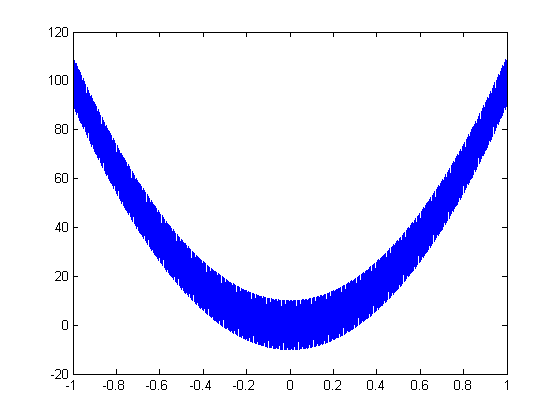
\includegraphics[width=0.5\linewidth]{GSA}
\caption{$y=(10x)^2 + 10 \sin(1000x)$}
\end{figure}
\noindent The global minimum is around -0.00157 where the function is -9.99975. The
value found by the algorithm is 0.02365 and the value of the function is
-9.902866. This result shows us that the method has the possibility of being applied
efficiently for multidimensional problem.
